\documentclass[notitlepage]{report}
\usepackage[utf8]{inputenc}
\usepackage[a4paper, margin=4cm]{geometry}
\usepackage{xcolor}
\usepackage{hyperref}
\usepackage{graphicx}

\title{Learning to Coordinate Autonomous Vehicles through Networks of Intersections using Neural Combinatorial Optimization}
\author{Jeroen van Riel}

\begin{document}

\maketitle
\begin{abstract}
  Coordination of autonomous vehicles through networks of
  intersections has the potential of reducing risk of accidents while providing
  huge savings in economic costs.
  %
  We adopt an optimal control formulation with hard collision-avoidance
  constraints as a model to study the fundamental complexity of centralized
  coordination schemes for autonomous traffic without traffic signals. With
  delay as the main performance criterion, we show that our problem decomposes
  into an upper-level problem that is a variant of the classical job-shop
  scheduling problem and a lower-level trajectory optimization problem that can
  be efficiently solved by linear programming.
  %
  Previous works have successfully proposed reinforcement learning methods to
  train scheduling policies based on the well-known disjunctive graph formalism
  of job-shop problems.
  %
  We propose to adapt this formalism to our job-shop variant and, like previous
  works, to use a graph neural network to parameterize a scheduling policy that
  is tuned using reinforcement learning in order to obtain a scalable
  approximation scheme for the high-dimensional coordination problem.
\end{abstract}


\begin{figure}
  \centering
  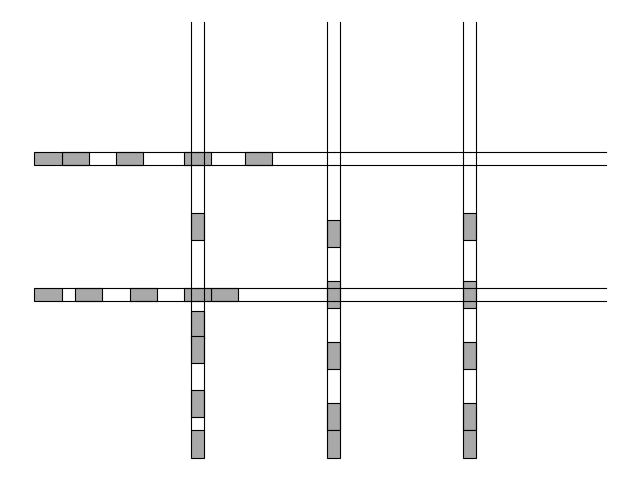
\includegraphics[width=0.55\textwidth]{figures/state_example.png}
  \caption{Illustration of some grid-like network of intersections with vehicles
    drawn as grey rectangles. There are five vehicle routes: two from east to
    west and three from south to north. Turning at intersections is not
    allowed.}\label{fig:network_illustration}
\end{figure}

\section*{Overall aim and goals}

\subsection*{Motivation and challenges}

% context and overall motivation
Given the ongoing development of self-driving vehicle technology, it is not hard
to imagine a future vehicular mobility system without human drivers. Besides the
obvious advantage of relieving us from the task of driving, freeing time that
can be spend on more meaningful activities, other benefits include increased
safety and efficiency. Human error is one of the major causes of most accidents
in vehicular traffic, which motivates the design of automated systems with
guarantees about collision avoidance, with the potential of saving millions of
injuries and lives. Furthermore, traffic coordination methods promise to reduce
economic costs such as travel delay, energy consumption and
pollution~\cite{fagnantPreparingNationAutonomous2015}.


% scope
We can identify different levels at which coordination can take
place~\cite{marianiCoordinationAutonomousVehicles2022}. At a local level,
platooning of vehicles may reduce energy consumption due to the reduced
aerodynamic resistance and may result in more efficient use of intersections. On
the other end of the spectrum, network-wide dynamic route optimization can be
employed to reduce the travel delay for all users of the system.
%
We choose to study a global model of coordination in which every vehicle in the
network is controlled by a single entity, to which we will simply refer as the
\textit{controller}. We ignore the choice of routes by assuming that each
vehicle follows a fixed predetermined route.

% main challenges
We identify the following two main challenges that are not fully addressed by
existing coordination schemes.
% collision avoidance by design
It is nontrivial to design systems that are guaranteed to be safe
with respect to collisions, because the potentially complex vehicle dynamics
must be taken into account.
% Ideally, the coordination controller follows a policy that is structured such that collision-avoidance constraints are respected by design.
% Alternatively, safety can be enfoced at inference time by employing some kind of look-ahead mechanism.
% scalability
Even when safety is guaranteed, optimal decision making is still a very
computationally challenging task due to the complex interactions and constraints
between vehicle trajectories that emerge in large traffic networks. Therefore,
an important research direction is the design of computationally efficient
coordination schemes with safety guarantees that scale to large networks with
large numbers of vehicles.
% robustness to uncertainty
Orthogonal to the above issues is the incorporation of assumptions that make the
coordination model more realistic. Most importantly, real-world systems should
be robust in terms of dealing with different forms of unexpected events. For
example, different kinds of failure in hardware or communication systems
complicate the design of systems with guarantees on safety and efficiency.

% RL success
Motivated by successful applications of reinforcement learning to highly complex
control tasks, we aim to apply a similar perspective to traffic coordination in
order to automatically learn how to deal with the complex decision-making problem.
% constraint satisfaction
However, it is nontrivial to apply current reinforcement learning formulations to
this setting, because satisfaction of hard constraints, like collision
avoidance, is still an area of active research
\cite{minHardConstrainedNeuralNetworks2024}.
% recent neural JSSP success motivates further investigation
We observe that traffic coordination shows some resemblance with classical
job-shop scheduling problems, for which successful reinforcement learning
methods have recently been proposed
\cite{zhangLearningDispatchJob2020,zhangDeepReinforcementLearning2024,smitGraphNeuralNetworks2024},
motivating the investigation of a similar approach to the current traffic
coordination problem.


\subsection*{Broad literature analysis}

Traffic lights are currently the most effective way of steering traffic, so
current coordination methods often rely on some sort of synchronization of
traffic light settings at neighboring intersections~\cite{mcshaneTrafficEngineering1990,hePAMSCODPlatoonbasedArterial2012}, with \textit{green waves} on
arterial roads being a well-known example. Since the complex interactions in
signalized networks are difficult to model explicitly, recent years have seen an
increased interest in the application of deep learning models to traffic-related
problems. In particular, numerous works have successfully proposed deep
reinforcement learning methods for traffic signal control that scale to large
networks of intersections~\cite{noaeenReinforcementLearningUrban2022,weiSurveyTrafficSignal2020}.
%
Furthermore, given the increasing number of fully autonomous vehicles, new types of traffic
coordination scheme become
conceivable~\cite{marianiCoordinationAutonomousVehicles2022}, with notable
examples being services like smart parking and ride sharing, local coordination
methods like ramp merging and platooning, or network-wide traffic flow
optimization through smart route suggestions.

Intersection access management without traffic signals is one type of setting in
which coordination of autonomous vehicles can potentially bring huge benefits,
both in terms of reduced risk and economic costs. While early works were mostly
based on reservation-based
protocols~\cite{dresnerMultiagentApproachAutonomous2008}, current coordination
schemes are studied under very different model assumptions regarding vehicle
dynamics and modes of communication and
control~\cite{khayatianSurveyIntersectionManagement2020}. An important
distinction can be made based on the used communication models, which can be
roughly categorized in distributed approaches, where groups of vehicles
coordinate trajectories together, and centralized approaches, where individual
vehicles receive instructions from a central controller.

Centralized solutions for access control at a single intersection have be
studied by framing the problem in terms of optimal control, providing a sound
theoretical foundation. Most works from this perspective use a simple
one-dimensional vehicle model known as the double integrator in optimal control
literature. Although solutions can be obtained using so-called \textit{direct transcription}
methods, the high-dimensionality of the problem calls for good approximation
schemes. A common observation is that the optimization problem may be thought of
as two coupled optimization
problems~\cite{hultApproximateSolutionOptimal2015,zhaoBilevelProgrammingModel2021,tallapragadaHierarchicaldistributedOptimizedCoordination2017},
where the upper-level problem is to determine when and in which order vehicles
enter and exit each intersection on their route. The lower-level problem is to
find optimal trajectories that match these time slots.

Extensions to multi-intersection settings have received much less attention.
Existing methods are extensions of reservation-based
protocols~\cite{hausknechtAutonomousIntersectionManagement} or are based on
mixed-integer linear programming~\cite{sartorCombinatorialLearningTraffic2019}.
% neural combinatorial optimization
We recognize that such a multi-intersection extensions is in large part of a
combinatorial nature. Recently, there has been an increasing interest in
applying a machine learning perspective on many classical combinatorial
problems~\cite{bengioMachineLearningCombinatorial2020}. Realistic instances of many combinatorial problems are often too
complex to solve to optimality, so researchers try to propose good approximation
schemes and heuristics, based on some kind of structure in the problems of
interest. However, manually designing such heuristics is a tedious task,
requiring a lot of experience and deep insight into the problem. Tailored deep
reinforcement learning methods have shown to be able to automatically derive
good heuristics from scratch for many classical combinatorial optimization
problems~\cite{mazyavkinaReinforcementLearningCombinatorial2020}.


\subsection*{Problem formulation and objectives}

% problem formulation
We are interested in centralized methods for network-wide coordination of
autonomous vehicles without relying on traffic lights. More precisely, we model
coordination as an optimal control problem, with assumptions of perfect
communication and control.
%
Imagine that some central coordinator controls the acceleration of all individual vehicles, each modeled as a double integrator.
After a vehicle arrives to the network, it follows a predetermined route and leaves
again.
The goal is to control the trajectory of each vehicle in the network while
avoiding collisions and optimizing some global measure of efficiency.
A natural measure of efficiency that is commonly used in literature is total delay experienced by
all vehicles.
However, it might be desirable to also penalize acceleration as a proxy
for energy consumption.
When all vehicle arrival times are known in advance, we
may assume that trajectories can be computed without any prior interaction with the
system, so we refer to this setting as \textit{offline trajectory optimization}.

Our overall goal is to investigate the limits of centralized coordination
algorithms in terms of performance and computational complexity.
Therefore, we state the following two research questions:
\begin{itemize}
  \item What are the fundamental limits on performance gains that centralized
        network-wide coordination of autonomous vehicles can bring?
  \item Is there any structure in the trajectory optimization problem that can be
        exploited by coordination algorithms?
\end{itemize}

To answer these questions, we propose to develop computationally efficient
coordination algorithms for the model skeched above. Results obtained in such
stylized models provide rough upper bounds on the performance gains we can
expect in a more realistic setting, where vehicle hardware and communication
systems are assumed to be less perfect.
%
More concretely, we aim to investigate how deep reinforcement learning can be
applied to the offline trajectory optimization problem, because we are convinced
that a data-driven perspective is beneficial in complex decision-making problems
(either deterministic or with uncertainty) where good policies are unlikely to
display simple structure.
% objectives
To this end, we propose to develop a coordination algorithm that satisfies the
following three key requirements:

\begin{itemize}
  \item \textit{Safety.} Because vehicle dynamics are assumed to be known precisely, hard
        collisions-avoidance constraints can be formulated, which the controller
        needs to respect at all times. Because safety is so crucial in
        real-world application, we feel it does not make sense to study
        algorithms without this guarantee.

  \item \textit{Scalability.} We want our coordination algorithm to naturally scale
        to complex networks with large numbers of vehicles in such a way that
        the required level of optimality can be achieved by providing sufficient
        computational resources.

  \item \textit{Learning.} The previous objective calls for the use of approximation schemes,
        because the computational complexity of the general coordination problem
        does not allow scalable solutions. Our hypothesis is that there is a lot
        of structure in the problem which can be algorithmically exploited, but
        might be hard to formulate precisely. Therefore, the algorithm must be
        able to automatically learn how to exploit the structure in some class
        of problem instances.
\end{itemize}


\section*{Research approach}

\subsection*{Overall methodology and decomposition}

% infinite dimensional -> direct transcription
Because trajectories are smooth functions, the offline trajectory optimization
problem is generally of infinite dimension. In order to solve it numerically,
some dimensionality reduction scheme is required. A straightforward way to
represent trajectories is based on a discrete time grid. Based on this, it is
possible to formulate a mixed-integer linear program, whose optimal solutions
approximate solutions to the original problem. Such so-called \textit{direct
  transcription} methods are very common for optimal control problems, but they
are still very high-dimensional due to the time discretization.

% bilevel decomposition
We show how the dimension can be reduced further, based on the following
observation. A key issue the coordinator has to decide is the order of crossing
at intersections, which is precisely what makes the optimal control problem
non-convex and thus hard to solve with standard methods. When considering an
optimization objective in terms of vehicle delay and some additional
assumptions, the problem can be shown to decompose as a \textit{bilevel} optimization
problem with an \textit{upper-level} combinatorial problem to determine a crossing time
schedule --- indicating when vehicles cross the intersections along their route
--- and a \textit{lower-level} optimal control problem to find trajectories that match
these crossing times, see Figure~\ref{fig:network_bilevel} for an illustration.

\begin{figure}[h]
  \centering
  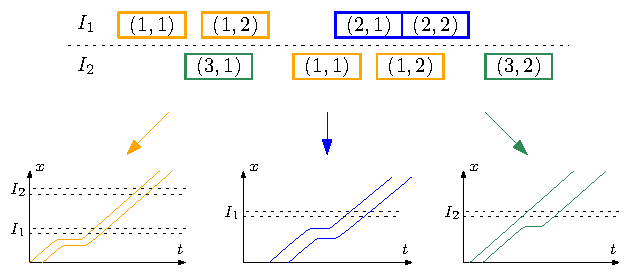
\includegraphics[width=1.0\textwidth]{figures/network_bilevel.pdf}
  \caption{Illustration of the proposed bilevel decomposition. The upper-level
    problem is assign each vehicle a time slot for each of the intersections
    (here denoted $I_{1}$ and $I_{2}$) on its route. Based on this schedule, the
    lower-level problem is to generate trajectories satisfying these time
    slots.}
  \label{fig:network_bilevel}
\end{figure}

% upper-level: job shop scheduling variant
Under some assumptions on the routes that vehicles take, it can be shown that
the upper-level problem, to which we will refer as the Vehicle Scheduling
Problem (VSP), is an extension of the classical Job-Shop Scheduling Problem
(JSSP). Intersections are modeled as machines (the shared resources) and each
vehicle corresponds to a job, whose operations model the crossing of
intersections along the vehicle's route.
%
In addition to the regular JSSP constraints, three types of additional
constraints are defined to model some necessary clearance time at intersections
and to take into account the travel time between intersections and safety
constraints to prevent rear-end collisions.
% lower-level efficient
Given a solution to the VSP, computing the lower-level trajectories can be done
reasonably efficiently, as we show in the next section. Furthermore, it can be
shown that trajectories that satisfy the schedule are guaranteed to
be collision-free, satisfying our first objective of guaranteed safety.
% focus on upper-problem
Therefore, the bilevel decomposition enables us to focus on solving the
scheduling problem.

% 1. MILP
Like plain JSSP problems, VSP can be solved by formulating it as a Mixed-Integer
Linear Program (MILP) and using an off-the-shelf solver. Although being a
powerful optimization framework, this approach is not likely to scale well,
because of the inherent complexity of larger instances. However, by setting a
time limit on the solving time, this method yields a good heuristic solution
method.

% 2. neural COP
To tackle the scalability issue, we propose to leverage the recent progress made
in applying Deep Reinforcement Learning (DRL) methods to Combinatorial
Optimization Problems (COP), of which JSSP is a classical example. We show that
the disjunctive graph encoding of job-shop problems can be extended to our VSP
variant. Following the approach of previous successful deep reinforcement
learning methods for job-shop problems, we propose a policy for generating
schedules in a step-by-step fashion. The policy is parameterized based on a
Graph Neural Network (GNN) encoding of the adapted disjunctive graph. We verify
whether the resulting policy space is general enough by using imiation learning
on expert demonstration obtained from optimal solutions by backtracking the
required step-by-step decisions. Finally, we train the policy using
reinforcement learning in a step-by-step scheduling environment.


\subsection*{Models and methods}

% We now provide a more detailed introduction of the most important models and
% methods that we plan to use and discuss how they can be adapted to the current
% problem formulation.

\subsubsection*{Trajectory optimization}

% vehicle dynamics and feasibility
The bilevel decomposition sketched above depends heavily on the feasibility of
the lower-level trajectory optimization problem. More precisely, we need to be
sure that a crossing time schedule always allows trajectories that respect the
vehicle dynamics and are collision-free.
% three different crossing snapshots
Therefore, we distinguish three key moments in time related to a particular
crossing. For some combination of an intersection and a vehicle with this
intersection on its route, let the \textit{crossing time} $y$ be the first
moment when the front bumper of the vehicle $i$ enters the intersection area, as
depicted by the first situation in Figure~\ref{fig:vehicle_crossing}. Next, let
$\rho > 0$ denote the time after which another vehicle on the same route can
start crossing and let $\sigma > \rho$ denote the of a \textit{full crossing},
which is time after which any vehicle from a conflicting routes can start
crossing the intersection.
% assumption on v=vmax on whole crossing time slot
To simplify matters, we assume that vehicles \textit{drive at full speed when
  crossing the intersection}, so for all $t$ between $y$ and
$y + \sigma$.

\begin{figure}[h]
  \centering
  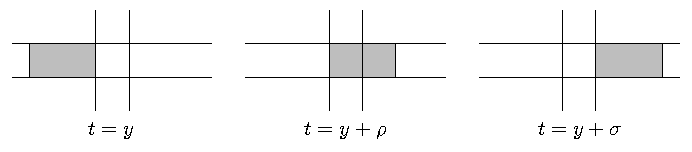
\includegraphics[width=0.85\textwidth]{figures/vehicle_crossing.pdf}
  \caption{Three different snapshots of a vehicle crossing an intersection.}
  \label{fig:vehicle_crossing}
\end{figure}

% separate optimal control problems per route
The upper-level scheduling problem provides the crossing times $y$,
which the trajectories must satisfy. Together with the constraints from the
double integrator vehicle dynamics, this yields a separate optimal control
problem for each group of vehicles with the same route.
% direct transcription
Each of these can be straightforwardly solved by direction transcription to a
linear program by introducing a discrete time grid to represent each vehicle's
trajectory. The vehicle dynamics can be encoded using a forward Euler scheme or
higher-order numerical integration methods. Rear-end collision-avoidance
constraints can simply be added for each timestep. Finally, the position at
timestep $y$ is bound to the start of the intersection.


\subsubsection*{Job-shop scheduling}

We briefly introduce the Job-Shop Scheduling Problem (JSSP), because we
formulate our Vehicle Scheduling Problem (VSP) as a direct extension. For a
textbook introduction, we recommend the very accessible book on scheduling by
Pinedo~\cite{pinedoSchedulingTheoryAlgorithms2016}.
%
The classical JSSP problem considers a set of $n$ jobs that must be assigned to
non-overlapping time slots on a set of $m$ machines. Each job $i$ has a set of
$n_{i}$ operations $O_{i1}, \dots, O_{in_{i}}$ that need to be executed in this
order. Each operation $O_{ij}$ requires $p_{ij}$ processing time on machine
$M_{ij}$. Each machine can process at most one operation and early preemption is
not allowed. The task of the scheduler is to determine a valid schedule of start
times $y_{ij}$ for each operation, while minimizing some objective function. Let
$C_{ij} = y_{ij} + p_{ij}$ denote the \textit{completion time} of operation $O_{ij}$.
Common optimization objectives are a function of these completion times, e.g.,
minimizing the total completion time among operations or minimizing the maximum
completion time, also known as the \textit{makespan}. Objectives that are a
non-decreasing function of completion times are called \textit{regular}.

% disjunctive graph
A commonly used representation of JSSP instances is the \textit{disjunctive
  graph}, with vertices $\{ O_{ik} : 1 \leq i \leq n, 1 \leq k \leq n_{i} \}$
corresponding to all the operations. The set of \textit{conjunctive arcs} encodes
all the precedence constraints $O_{i,k} \rightarrow O_{i,k+1} $ among each job's
operations. The set of \textit{disjunctive edges} consists of undirected edges
between each pair of operations from distinct jobs that need to be processed on
the same machine, effectively encoding all such \textit{conflicts}. Each valid
schedule induces an ordering of operations on machines that is encoded by fixing
the direction of each disjunctive edge such that we obtain a directed acyclic
graph.

\begin{figure}[h]
  \centering
  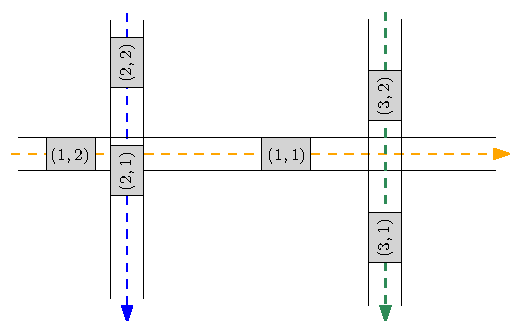
\includegraphics[width=0.65\textwidth]{figures/network_indices.pdf}
  \caption{Example network with three different routes satisfying the
    edge-disjoint assumption (such that vehicle flows never merge) and vehicle
    indices $(r,k)$.}
  \label{fig:network_indices}
\end{figure}

We now explain how JSSP can be extended to our Vehicle Scheduling Problem (VSP),
where intersection are modeled as machines, vehicles correspond to jobs.
% network graph, crossing <-> operation
The road network is represented as a simple directed graph with nodes
representing intersections. Each vehicle has a fixed route consisting of a
series of intersections. The act of \textit{crossing} an intersection along this
route is modeled as an operation. The processing time of a crossing corresponds
to $\rho$ in Figure~\ref{fig:vehicle_crossing}.
% edge-disjoint routes, no overtaking => (r,k) indices
We assume that routes are \textit{edge-disjoint}, in the sense that they do not
share edges but may possibly overlap at nodes (intersections). Furthermore, we
assume that vehicles on the same lane are not able to overtake. Therefore, each
vehicle can be identified as a tuple $(r, k)$, with some route identifier $r$
and an integer $k$ that indicates the relative order on this route, see
Figure~\ref{fig:network_indices} for an example. In addition to the regular
constraints of JSSP, we define the following three constraints:

\begin{itemize}
  \item \textit{Clearance time.} To guarantee collision-free crossing at
        intersections, some additional time is required between crossing times
        for vehicles that approach an intersection from different lanes. More
        precisely, we require at least $\sigma$ time (see
        Figure~\ref{fig:vehicle_crossing}) between crossings of vehicles
        belonging to different routes.

  \item \textit{Travel constraints.} Vehicles need to physically drive towards
        the next intersection along their route, so there is a lower bound on
        the travel time. Therefore, we need a constraint between the crossing
        times at every two consecutive intersections on each vehicle's route.

  \item \textit{Buffer constraints.} Each lane between intersections has only
        space for a limited number of vehicles, depending on their position and
        velocity. To avoid rear-end collisions, the number of vehicles in each
        lane needs to be limited.
        %
        This type of constraint is the most difficult to formulate, so the basic
        principle is illustrated by the example in
        Figure~\ref{fig:buffer_constraints}.
\end{itemize}

\begin{figure}[h]
  \centering
  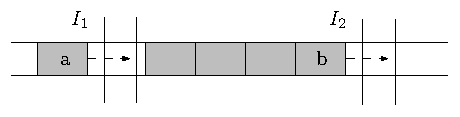
\includegraphics[width=0.6\textwidth]{figures/buffer_constraints.pdf}
  \caption{Illustration of buffer constraint for a pair of vehicles on the same
    route. Suppose that the vehicles on the lane between the two intersections
    are currently not moving and waiting to cross $I_{2}$. It is clear that the
    crossing time of vehicle $a$ at $I_{1}$ must be happen at least after
    vehicle $b$ starts crossing $I_{2}$. Since this particular lane segment has
    capacity for 4 waiting vehicles, we need such a buffer constraint between
    every pair of vehicles $(r,k_{1})$ and $(r,k_{2})$ that satisfy
    $k_{2} = k_{1} + 3$.}
  \label{fig:buffer_constraints}
  \end{figure}

%{\color{blue} discuss simple heuristics (based on priority rules)}

\subsubsection*{Mixed-integer linear programming}

% mixed-integer programming
Like the original JSSP, our VSP can be formulated as a Mixed-Integer Linear
Program (MILP).
% single intersection
For a single isolated intersection, it is very straightforward to do this. The
crossing order decisions can be modeled by introducing a binary decision
variable for each pair of conflicting vehicles that approach the intersection
from different lanes. Note that the number of these so-called
\textit{disjunctive decisions} grows exponentially in the number of vehicles.
% platoon preservation
Whenever two consecutive vehicles on the same lane are able to cross the
intersection without a gap, it has been shown that they will always do so in any
optimal schedule~\cite{limpensOnlinePlatoonForming2023} (with respect to the
total delay objective).

% network: addresses scalability objective
When considering a network of intersections, the two additional types of constraints
are necessary to guarantee feasibility of the lower-level trajectory
optimization.
% both constraints can be encoded in disjunctive graph
Both constraint types can be naturally encoded in the disjunctive graph.
%
When we assume that there is no merging of routes, which means they only overlap
at intersections, we expect that VSP is still computationally tractable for
reasonably sized instances, using modern solvers. Whenever general routes
are considered, a naive formulation would include a lot of disjunctive
decisions, because vehicles can in principle conflict with all other vehicles
that share a part of their route, even if it is clear that this would never
happen in any sensible schedule.

During the solving procedure, the currently best solution is remembered.
Therefore, MILP solving can be used as an approximation method by setting a
limit on the computation time, which addresses our second overall objective.
%
Another benefit of the MILP framework is the easy incorporation of
problem-specific \textit{cutting planes} in order to exploit additional
structure in problem instances. For example, we observe that the above property
on crossing without a gap in a single intersection can be used to formulate
multiple types of cutting planes to improve the running time of the solver.


\subsubsection*{Constructive neural heuristic}


% neural combinatorial optimization
We now explain how to model VSP as a sequential decision making process such
that deep reinforcement learning can be applied to address our objective of
obtaining a learning optimization algorithm.
% determine crossing order
The fundamental challenge of the scheduler is to determine in which order
vehicles are allowed to cross the intersections along their routes. Observe that
the relative order among vehicles on the same route stays fixed, because they
are not allowed to overtake.
%
We propose to order vehicles in a step-by-step fashion. For each intersection,
we keep track of a partial ordering of vehicles. Each step corresponds to
choosing some combination of an intersection and a vehicle that has not yet been
added to the partial ordering of this intersection and has this intersection on
its route. We will refer to such intersection-vehicle pair as a \textit{crossing}.
Figure~\ref{fig:network_ordering} illustrates an example of a partial ordering after four steps.

\begin{figure}[h]
  \centering
  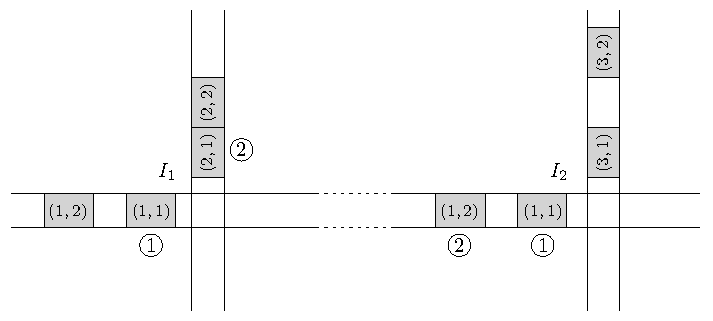
\includegraphics[width=0.9\textwidth]{figures/network_ordering.pdf}
  \caption{Illustration of some partial ordering, indicated by the encircled
    numbers. The order among vehicles without an encircled number is still to be
    decided by the scheduler, bust must respect the fact that vehicles on the
    same route cannot overtake. In this particular example, this means that the
    crossing order at $I_{2}$ can only be completed in one way.}
  \label{fig:network_ordering}
\end{figure}

This step-by-step process can be cast into the Markov Decision Process (MDP)
framework.
% state is partial ordering and action is (intersection, vehicle) pair
The state corresponds to the current partial ordering and each action
corresponds to a valid intersection-vehicle pair to add to the partial ordering.
Observe that the MDP is completely deterministic by definition. As we will show
next, a complete ordering of vehicles induces a complete schedule with exact
crossing time slots, so we may simply define an episodic reward in terms of the
total delay of the final schedule.
% disjunctive graph to encode partial ordering
The disjunctive graph, see Figure~\ref{fig:disjunctive_graph}, provides a way to
encode a partial ordering by specifying the direction of a selection of
disjunctive edges.
% lower bounds in partial disjunctive graph
Using the resulting \textit{partial disjunctive graph} we can derive lower bounds on the crossing
times. Recall that every node of the disjunctive graph corresponds to a crossing
and that every arc corresponds to some constraint. We can derive lower bounds on
the crossing times based on all the constraints whose arc has been added to the
partial disjunctive graph by solving a linear program.
% efficient LB update
However, we think that it is possible to develop a tailored update scheme that
only propagates the necessary changes over the partial disjunctive graph
whenever a set of disjunctive arcs is added.
% complete ordering => complete schedule
Finally, it is not difficult to see that the lower bounds for a complete ordering are
precisely the crossing times of the corresponding schedule.

\begin{figure}[h]
  \centering
  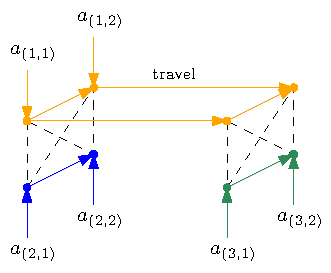
\includegraphics[width=0.6\textwidth]{figures/disjunctive_graph.pdf}
  \caption{Illustration of a disjunctive graph corresponding to the instance in
    Figure~\ref{fig:network_bilevel} with respect to the network from
    Figure~\ref{fig:network_indices}. For each route, conjunctive arcs are drawn
    at a slight angle and the horizontal arcs correspond to the travel
    constraints (only applicable to vehicles on route 1). The dashed lines
    represent disjunctive edges for the two intersections. For each node
    corresponding to the first intersection on the route $r$, an incoming arc
    labeled $a_{(r,k)}$ represents the earliest arrival time constraints. Buffer
    constraints are not shown, as they are not applicable to this small
    example.}
  \label{fig:disjunctive_graph}
\end{figure}

We will now discuss how to parameterize the scheduling policy, which is a
function from a partial solution (partial disjunctive graph) to an action
(crossing).
% disjunctive graph -> GNN -> encoding of partial solution
Previous works have been able to train good policies based on encodings of the
disjunctive graph for JSSP. Following this direction, we propose build
an encoding of the partial disjunctive graph augmented with the corresponding
crossing time lower bounds.
%
Graph Neural Networks (GNN) are deep neural networks that are suited to encode
graph-structured data from node-level features. For each node in the (partial)
disjunctive graph, we record two basic features: (i) a binary variable
indicating whether this crossing has already been scheduled and (ii) the current
crossing time lower bound. By iteratively combining these node-level features in
a parameterized non-linear fashion, we obtain an embedding $h_{O}$ for every
node $O$ and a global graph embedding $O_{\mathcal{G}}$. These embeddings are
then mapped to an action distribution via a fully connected net and softmax
function.
% size-agnostic
As already noted in~\cite{zhangLearningDispatchJob2020}, such an architecture has the major advantage of being
size-agnostic, meaning that the same policy can be applied to other instances
with a different network and varying number of vehicles.

% imitation learning
We will consider two learning paradigms for tuning the parameters in order to
obtain good policies. In the \textit{imitation learning} setting, the policy is
trained to imitate expert demonstration. For example, we can use a MILP solver
to obtain the optimal schedule and then backtrack the corresponding state-action
pairs that our policy must take in order to arrive at the same schedule. These
resulting training set of state-action pairs can then be used to tune the policy
in order to mimic the expert policy as closely as possible.
% reinforcement learning
When expert demonstration is not available, we can directly learn from
interaction with the MDP, which is what is generally known as \textit{reinforcement
  learning}. Policy parameters are tuned using a policy gradient
learning algorithm like the classical REINFORCE~\cite{10.1007/BF00992696} or the
more recent Proximal Policy Optimization
\cite{schulmanProximalPolicyOptimization2017}.


\subsection*{Research plan and timeline}


Time estimates are based on a total duration of 20 weeks of which the last two
weeks are reserved for report writing and preparing material for a final
presentation.

\begin{itemize}
  \item (done) \textbf{Direct transcription of lower-level.} The proposed bilevel
        decomposition depends heavily on our ability to solve the lower-level
        problem efficiently. Therefore, our first effort should be to develop a
        working direct transcription solution to obtain trajectories for a given
        crossing time schedule.

  \item (2 weeks) \textbf{Upper-level formulation.} We precisely formulate VSP for
        networks with delay objective (network scheduling problem).
        Particularly, this mainly involves formulating the travel constraints
        and buffer constraints such that feasibility of the lower-level problem
        is guaranteed. At this stage, we only aim to provide a rough proof
        sketch of this, because we simply verify this feasibility

        %{\color{blue} We are almost done with this, the only missing part is a clear argument
        %of why we expect our current version of buffer constraints to work.}

  \item (done) \textbf{MILP for VSP.} Solve the network scheduling problem by formulating and
        solving it as a MILP. This method can be used to collect expert
        demonstrations for training the neural scheduler using imitation
        learning and it also provides a baseline for peformance evaluation of
        our proposed neural scheduler.

  \item (3 weeks) \textbf{MDP scheduling formulation.} As a first step towards implementing
        the actual neural scheduler, we precisely formulate the constructive
        combinatorial optimization in terms of a Markov Decision Process. Next,
        we implement a simulation of this MDP (or \textit{environment}) that we will
        use to train and test our policies.

  \item (2 weeks) \textbf{Augmented disjunctive graph.} Next, we focus on the policy
        parameterization based on the disjunctive graph. First, we show how to
        augment the disjunctive graph with lower bounds on starting times. Each
        time a scheduling step is taken, the lower bounds can be efficiently
        recomputed using a message-passing scheme over the disjunctive graph,
        where the number of required messages is limited. After formulating this
        message-passing scheme, we prove correctness before writing the
        implementation.

  \item (3 weeks) \textbf{GNN encoding.} Based on the augmented disjunctive graph, we design
        a suitable embedding to parameterize the policy. We do not have much
        experience with the representational power of graph neural networks, so
        we plan to first consult the available literature to make an informed
        choice about the specific architecture to use. In particular, we know
        that not all graph neural networks are able to distinguish different
        graph structures, which we need for our purposes.

  \item (2 weeks) \textbf{Imitation learning.} Fit the policy to expert demonstration
        obtained from the MILP solver. We first need to extract state-action
        pairs from optimal solutions by some straightforward backtracking
        procedure. Next, we formulate and implement the corresponding supervised
        learning problem.

  \item (2 weeks) \textbf{Reinforcement learning.} Next, we decide on a suitable
        policy gradient method and we implement the main reinforcement learning
        training loop. This should be a simple coding exercise, since we already
        have a working environment at this point.

  \item (2 weeks) \textbf{Policy evaluation.} We design a series of numerical experiments to
        assess the performance of the learned scheduling policy. In order to
        make a fair comparison, we set a time limit on the MILP solver and
        compare schedules generated by our trained policy to those obtained from
        simple priority rules and those found by the MILP solver.
        %
        Furthermore, since our policy is size-agnostic by design, we study how
        well the trained policy generalizes to instances with larger networks
        and larger number of vehicles.

  \item (2 weeks, not essential) \textbf{Explicit trajectories.} We would like to
        derive explicit trajectories for the lower-level trajectory optimization
        problem, which might be used in the future to show that the
        decomposition is sound, rigorously proving that valid schedules always
        lead to feasible lower-level problems.
\end{itemize}



\subsection*{Identified risks and their mitigation}

% We identify the following risks, shown in order of impact on our research.
It may turn out that our formulation of VSP does not always yield feasible
lower-level problems. This can easily be verified empirically once we have a
working implementation of the lower-level trajectory planning and some basic
scheduling algorithm (or heuristic rule) to generate random example schedules,
for which we try to compute trajectories. When some of these lower-level
problems turn out to be infeasible, it is very likely that this is due to the
buffer constraints, for which it is nontrivial to argue correctness. A possible
solution to try in this situation is to tighten the buffer constraints, meaning
that we further restrict the number of allowed vehicles between intersection.

Once we start considering the crossing time scheduling problem in networks, it
is not guaranteed that even modern MILP solvers will find optimal solutions for
small instances. This is a problem, because we would like to use the MILP
technique as a baseline in the analysis of our neural scheduler and for
obtaining expert demonstration for imitation learning. In any case, we might
choose a fixed MILP optimality gap to obtain approximate schedules in limited
time, or we could use simple priority rules instead.

% trained model not satisfactory
We aim to train scheduling policies that provide reasonably good schedules in
limited time for large networks and hopefully to outperform MILP-based
heuristics. We expect that potential issues are mostly related to model capacity
and training time.
% not enough capacity
First, it might be the case that our model has not enough representational power
(model capacity) to capture the complex dynamics required for good policies. In
other words, it is not guaranteed that the resulting total space of possible
policies does not include optimal policies or near-optimal policies. For
example, it is well known that graph neural networks may differ considerably in
representational power, depending on their exact
formulation~\cite{xuHowPowerfulAre2019}.
%
Therefore, we choose to first do imitation learning on expert demonstration. If
this yields policies with satisfactory performance (in terms of generated
schedule quality), we can have some confidence that the policy space is complex
enough to yield good policies with reinforcement learning.
% long training time
Even if the model has enough representational power, reinforcement learning
might show very slow convergence. To tackle this, we could opt to implement the
$n$-step REINFORCE algorithm proposed in~\cite{zhangDeepReinforcementLearning2024}.


We mentioned in passing that we think a tailored update scheme is possible for
calculating the starting time lower bounds from the disjunctive graph. Although
we have a rough idea of how this would work, we did not have enough time to
formulate our idea and provide arguments for it could work. However, we can
obtain the lower bounds by just solving the linear program, which we expect is
not too expensive to run at every transition of the reinforcement learning loop.

\subsection*{Discussion and further directions}


\textit{Why not model the coordination problem in terms of time steps?}
%
It is not difficult to image a time-step based model of vehicle movement through
a network of intersections, which is the main principle of traffic
micro-simulators like SUMO~\cite{lopezMicroscopicTrafficSimulation2018}. Actions may be defined in terms of increasing
and decreasing the acceleration of individual vehicles and we could consider the
corresponding \textit{joint acceleration action} for all vehicles in the network.
%
The main problem with this parameterization of trajectories is that safety is
not guaranteed by design. Without additional constraints, it is possible that
some sequence of joint acceleration actions eventually lead to collision. This
means that the set of allowed joint actions should change with the current
state.
%There is a lot of literature on \textit{safe reinforcement learning} methods.
%
In addition to this feasibility problem, any end-to-end method that uses
model-free reinforcement learning in such time step-based environment is
inherently sample-inefficient, because it would implicitly be learning the
vehicle dynamics, which is unnecessary.
%
Moreover, we think that there is much more to gain by coordination on a higher
level. The macroscopic phenomena that naturally occur in networks of
intersection, such as the emergence of platoons, are better modeled with this
higher level of abstraction.

\vspace{0.5em}\noindent
\textit{Full speed crossing.} For general objective functions involving some
measure of energy consumption, for example in terms of acceleration, it is not
always optimal to require vehicles to cross intersections at full speed. In
particular, previous works that treat a similar proplem with only a single
intersection~\cite{hultApproximateSolutionOptimal2015,zhaoBilevelProgrammingModel2021}
do not make this explicit assumption. However, we propose to focus first on the
higher-level decision of crossing order, because we think this has most impact
on the overall quality of trajectories. Nevertheless, it remains an interesting
direction for further investigation to extend our method to also allow different
crossing speeds.

\vspace{0.5em}\noindent
\textit{Explicit trajectory expressions.}
% lower-level explicit expressions
It can be observed that the resulting trajectories satisfy so-called
``bang-bang'' control, which means that the control input only takes both
extreme values (maximum acceleration, maximum deceleration) and zero (no
acceleration), in this case. Therefore, we think that it should be possible to
derive expressions for the time intervals during which these three control
inputs are active, as a function of the crossing times.
%
Such explicit expressions would also help towards rigorously proving soundness
of the bilevel decomposition, for which we would have to show that the
lower-level problem is feasible for every valid crossing time schedule.

\vspace{0.5em}\noindent
\textit{Stochastic modeling.}
It is not always realistic to assume future arrivals to the network are known
ahead of time. Instead, we assume vehicle arrive according to some (unknown)
random process, which means that current trajectories may need to be
reconsidered whenever a new arrival happens. Therefore, we refer to this setting
as \textit{online control}, where the focus is on finding optimal \textit{control policies} that
specify how to update trajectories over time.
% Miculescu and Karaman
%
For the online control problem with a single intersection and delay objective,
the paper~\cite{miculescuPollingsystemsbasedAutonomousVehicle2016} discusses a
model based on a similar bilevel decomposition as discussed above. Whenever a
new vehicle arrives to some control area, the proposed algorithm simulates the
behavior of a polling policy to determine the new vehicle crossing order. It is
shown that it is always possible to compute a set of collision-free trajectories
from the updated schedule. Moreover, for certain classes of polling policies,
explicit trajectory expressions (also refered to as \textit{speed profile
  algorithms}) are available~\cite{timmermanPlatoonFormingAlgorithms2021}.

% online with re-optimization

A straightforward approach to the online problem in a single intersection would
be to re-optimize the crossing time schedule each time a new vehicle arrives.
However, the updated schedule should always have a feasible lower-level problem,
so we need to define constraints that take into account the fact that vehicles
cannot stop or accelerate instantaneously. It has been shown that the
feasibility of the lower-level optimization is guaranteed when the schedule is
updated based on the polling policy simulation
of~\cite{miculescuPollingsystemsbasedAutonomousVehicle2016}, but we think that
it is possible to achieve more freedom in the update step, which would allow
schedules to reach closer to optimality.


\bibliography{../references}
\bibliographystyle{ieeetr}

\end{document}
